% Written by make_deck_figures.py: edit the script, not this file.
% 130/30 weights of two made-up basket tickers and one short candidate.
\documentclass[tikz,border=2pt]{standalone}
% Shared style for the L15a schematics, copied from L14a (November 19, 2026), \input by each Fig-L15a-*.tex.
% Copied from week-13/L13a/figs/jumphmm-diagram.tex (the week-12 schematic style): same fonts,
% ink, accent colors, boxes, and arrows, plus a monospace font for tool names and order
% statuses. The notebook SVG carries a dark palette added by theme_svg.py; every color here
% must be mapped there.
\usepackage[no-math]{fontspec}
\IfFontExistsTF{Arial}{\setsansfont{Arial}}{\setsansfont{TeX Gyre Heros}}
\renewcommand{\familydefault}{\sfdefault}
\IfFontExistsTF{Menlo}{\setmonofont[Scale=0.92]{Menlo}}{}
\usepackage{amsmath,amssymb}
\usetikzlibrary{arrows.meta,calc,positioning,decorations.pathreplacing}

\definecolor{vnink}{HTML}{202124}
\definecolor{gdblue}{HTML}{0091FF}
\definecolor{gdred}{HTML}{E02020}
\definecolor{gdgray}{HTML}{6D7278}
\definecolor{saorange}{HTML}{F08C00}
\definecolor{boxfill}{HTML}{F1F3F4}
\definecolor{orangefill}{HTML}{FFE8C7}
\definecolor{bluefill}{HTML}{E5F3FF}
\definecolor{redfill}{HTML}{FDE8E8}
\definecolor{gridgray}{HTML}{E3E5E8}

\tikzset{
  every picture/.append style={x=1cm, y=1cm, font=\sffamily\small, text=vnink},
  % boxes and arrows, as in the L12a schematics
  flow/.style={draw=vnink, line width=0.9pt, -{Latex[length=2.4mm, width=1.7mm]}},
  feedback/.style={draw=saorange, line width=1.2pt, -{Latex[length=2.6mm, width=1.9mm]}, rounded corners=6pt},
  sumbox/.style={draw=vnink, fill=boxfill, line width=0.8pt, rounded corners=3pt, inner sep=5pt, align=center},
  note/.style={text=gdgray, font=\sffamily\footnotesize, align=center},
  state/.style={circle, draw=vnink, fill=white, line width=1.0pt, minimum size=1.1cm, inner sep=0pt, font=\sffamily\normalsize},
  % plots, as in the L10b profit diagrams
  axis/.style={draw=vnink, line width=0.8pt, -{Latex[length=2.6mm, width=1.8mm]}},
  spine/.style={draw=vnink, line width=0.8pt},
  curve/.style={draw=vnink, line width=1.6pt, line join=round, line cap=round},
  series/.style={draw=gdgray, line width=0.9pt, line join=round},
  drop/.style={draw=gdgray, line width=0.8pt, dash pattern=on 3pt off 2pt},
  pt/.style={circle, draw=vnink, fill=white, line width=1.0pt, inner sep=0pt, minimum size=2.0mm},
}


\begin{document}
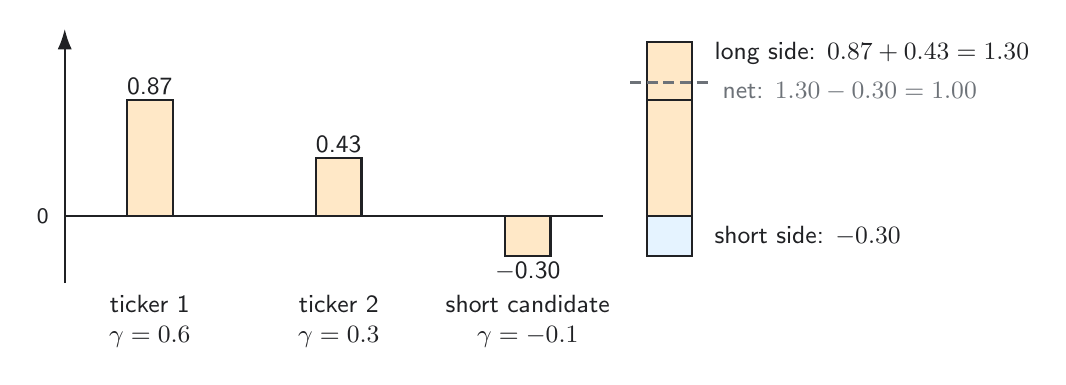
\begin{tikzpicture}
  \draw[axis] (0, -0.85) -- (0, 2.38);
  \draw[spine] (0, 0) -- (6.84, 0);
  \node[anchor=east, font=\sffamily\footnotesize] at (-0.08, 0) {0};
  \node[font=\sffamily\small, align=center, anchor=north] at (1.08, -0.88) {ticker 1\\$\gamma=0.6$};
  \filldraw[fill=orangefill, draw=vnink, line width=0.8pt] (0.79, 0) rectangle (1.37, 1.4733);
  \node[font=\sffamily\small, anchor=south, inner sep=2pt] at (1.08, 1.4733) {0.87};
  \node[font=\sffamily\small, align=center, anchor=north] at (3.48, -0.88) {ticker 2\\$\gamma=0.3$};
  \filldraw[fill=orangefill, draw=vnink, line width=0.8pt] (3.19, 0) rectangle (3.77, 0.7367);
  \node[font=\sffamily\small, anchor=south, inner sep=2pt] at (3.48, 0.7367) {0.43};
  \node[font=\sffamily\small, align=center, anchor=north] at (5.88, -0.88) {short candidate\\$\gamma=-0.1$};
  \filldraw[fill=orangefill, draw=vnink, line width=0.8pt] (5.59, 0) rectangle (6.17, -0.51);
  \node[font=\sffamily\small, anchor=north, inner sep=2pt] at (5.88, -0.51) {$-$0.30};
  \filldraw[fill=orangefill, draw=vnink, line width=0.8pt] (7.39, 0) rectangle (7.97, 1.4733);
  \filldraw[fill=orangefill, draw=vnink, line width=0.8pt] (7.39, 1.4733) rectangle (7.97, 2.21);
  \filldraw[fill=bluefill, draw=vnink, line width=0.8pt] (7.39, 0) rectangle (7.97, -0.51);
  \draw[draw=gdgray, line width=1.0pt, dash pattern=on 4pt off 2pt] (7.18, 1.7) -- (8.18, 1.7);
  \node[font=\sffamily\small, anchor=west, align=left] at (8.13, 2.074) {long side: $0.87+0.43=1.30$};
  \node[font=\sffamily\small, text=gdgray, anchor=west, align=left] at (8.23, 1.581) {net: $1.30-0.30=1.00$};
  \node[font=\sffamily\small, anchor=west, align=left] at (8.13, -0.255) {short side: $-0.30$};
\end{tikzpicture}
\end{document}
